

\documentclass[sigconf]{acmart}
\renewcommand\footnotetextcopyrightpermission[1]{}
\usepackage{graphicx}
\usepackage{titlesec}
\title{Forking Attacks: Two Ways, No Worries}
\author{Matija Roncevic}
\email{matija.roncevic@fau.de}
\affiliation{
    \institution{Friedricht-Alexander-Universität Erlangen-Nürnberg}
    \country{}
    \city{}}
\makeatletter

\let\@authorsaddresses\@empty 
\makeatother
\pagestyle{plain}
\settopmatter{printacmref=false}
\settopmatter{printfolios=false}
\bibliographystyle{plain}

\setlength{\parindent}{0pt} %%stoppt die Einrückung

\titleformat{\subsubsection}
  {\normalfont\normalsize\bfseries}{\thesubsubsection}{1em}{}

\begin{document}

\maketitle  % Dieser Befehl erzeugt den Titel, Autor und Datum im Dokument


\acmConference[FAU]{Bal bal bla}{June 2020}{Erlangen, Germany}

%%%%Für die Seitennummerierung
%%\thispagestyle{plain} %%damit auch die erste seite eine 1 hat
%%\pagenumbering{arabic}
%%\pagestyle{plain} %%???

\section{Abstract}
Nowadays, there is a great demand to outsource parts of systems. The term for digital outsourcing is cloud computing. With the advantages of cloud computing come new vulnerabilities. Outsourcing increases the attack surface and companies have already developed many concepts to prevent attacks. Intel, for example, implemented Software Guard Extension (SGX) to increase the security of Trusted Execution Environments (TEEs). However, SGX is also vulnerable to attacks.\\
In this paper, we look into forking attacks and two extensions that take different approaches to create an environment robust against forking attacks. The extensions have their own approaches which of course have different requirements, dependencies, and complexity. These approaches are analyzed and compared to identify possible applications and create added value that increases the reliability of cloud computing.


\section{Introduction}

Almost every noteworthy application has embraced cloud computing. The range of applications that benefit from cloud services spans from small smartphone apps to sophisticated large language models to commonly used GitHub repositories. The clear reason for its popularity is the ability to store, manage, and process data more efficiently than ever before. The shift to cloud services offers numerous advantages, including scalability, flexibility, and cost-effectiveness. However, it also introduces significant security challenges. With the inclusion of numerous critical applications and sensitive data, the importance of secure environments has increased. Cloud security involves a diverse range of practices, technologies, and policies aimed at protecting data, applications, and services distributed across cloud environments. Basic protection comes from using firewalls and encryption, but cyber threats are getting so advanced and constantly changing that these measures can't always keep up. This calls for advanced security solutions that can ensure the integrity of data even in potentially compromised environments.\\

Trusted Execution Environments (TEE) like Intel Software Guard Extensions (SGX) is such an advanced security solution. Intel SGX is a set of hardware-based security features that create isolated execution environments, known as enclaves (Enclaves -  areas of memory where sensitive data and code can be executed and stored in isolation from the rest of the system.)~\cite{nfw}. These enclaves are designed to protect sensitive data and code from being accessed or modified by unauthorized parties, even if the operating system is compromised. SGX provides a robust mechanism for ensuring the confidentiality and integrity of data processed in the cloud. Despite its strengths, Intel SGX still has its vulnerabilities. The enclaves themselves are in fact isolated from adversaries, however, the reliability of the input can not be ensured without additional safety measures. So a malicious OS could feed the enclave stale input data, to restore a passed state. Those attacks are labeled as rollback attacks~\cite{esccc}. \\
Forking attacks, on the other hand, aim to create multiple instances of an enclave (Clone), leading to unauthorized data access and manipulation. This is accomplished by running the enclave and the clones simultaneously and exploiting the fact, that all those instances will return correct but stale states. I.e. counters for password attempts can be reset to gain unlimited tries, despite the limit for tries being set to a finite number. Understanding these attacks and developing effective mitigation strategies is essential for ensuring the security and trustworthiness of cloud-based applications relying on SGX.

---------------------------------- Grammarly checked ---------------------------------------

\section{Background}

The following section will provide further knowledge about different aspects, covered in this paper.

\subsection{Trusted Execution Environment, TEE}

TEEs are designed to increace data security and prevent tampering with critical code sections. They achieve this by applying various protective mechanisms, such as the Intel SGX enclave system. The processor is, in those systems, provided with several memory areas which are ensured to be separate and safe from unauthorized access. This memory space is either detached by hardware or by software provided by Intel SGX. Sections of a program that execute critical operations, such as incrementing essential counters, are executed within these protected environments to ensure their security.
Furthermore, adversaries can not read or modify data saved inside this memory since it is encrypted.

\subsection{Attacks}

This paper aims to provide an overview of two methods to protect systems against forking attacks. However, the creators of those systems also included further attacks which we want to mention as well. These attacks come along when talking about forking and enclaves.

\subsubsection{Denial of Service (DoS) Attacks}
These attacks differ from the following attacks since the goal here is not to force the system to outputs that deliver advantages to the adversary by feeding in special inputs or launching several instances. DoS attacks rather overflow the system to disable services or downgrade service performance until the system shuts down and, as the name states, deny the completion of certain services~\cite{DoS}.

\subsubsection{Rollback Attacks}
Almost any system with a lifecycle can be rolled back to an outdated state, so an attacker can exploit the output to their advantage. Encalves are not the only targets for those kinds of attacks, VM for example are vulnerable to snapshots. These snapshots can be saved if e.g. certain restrictions on participants are not yet assigned and if needed this snapshot can be executed so this participant can bypass security measures and read information that it should not have access to~\cite{Rollback}. 

\subsubsection{Forking Attacks}
When an adversary creates several clones of an instance (e.g. an enclave) and launches them into the system, it is labeled as a forking attack. This attack exploits some vulnerabilities that are delivered, e.g. if these clones then try to connect again to the group in which its origin instance is running, it enables the clone to link to other groups as well, as discussed in §4.1.3. 
To show the connections between forking and rollback attacks it is important to mention that rollback attacks are often performed on clones of a forking attack. Since the clones deliver the opportunity to feed them stale inputs to receive outputs that bypass different security measures, like limited password attempts. So due to the connection of both attacks, the prevention of forking attacks leads to a certain prevention of rollback attacks as well. \\

DoS Attacks, on the other hand, are not aimed to be prevented by both methods, as stated later on. However, we decided to include the definition as well since they are discussed after all. \\


---------------------------------- Grammarly checked ---------------------------------------





\section{The Blockchain approach - Narrator-Pro}
 

This system~\cite{esccc} relies on an external blockchain to initialize certain components. The system itself can be broken down into three main concepts which combined yield in its prevention of attacks. The goals that are ensured are described as:
\begin{itemize}
     \item \textbf{Security} - The ~safety~ and ~liveness~ properties of the TEE programs will be guaranteed.
     \item \textbf{Performance} - Achieving the security goals will not significantly impact performance. In detail, the aim is low latency for state updates and read operations, high throughput for processing enclave program requests, and unlimited state updates, provided by the blockchain.
\end{itemize} 
To start this section it is essential to mention that Narrator-Pro considers a distributed system if it at least holds \textit{n} = 2\textit{f} + 1 SGX-enabled instances in a cloud. Where \textit{f} is the number of faulty State Enclaves, so the system can still properly work. The system can run a number (limited by specifications of the system) of enclaves which are divided into two groups of Application Enclaves (AEs) and State Enclaves (SEs). AEs have applications running, handle client requests, and return outputs corresponding to their inputs. SEs on the other hand contain the Narrator-Pro software and are responsible for providing state continuity to AEs. This is accomplished by a secure connection from the AE to a locally running SE, where the AE can use SEs Narrator-Pro libraries to seal data. This data is then used to retrieve the latest sealed state, in case of unexpected shutdowns. This principle is explained in more detail in §4.2. Figure ~\ref{fig:1} provides an overview of the mentioned components.

\begin{figure}[h]
    \centering
    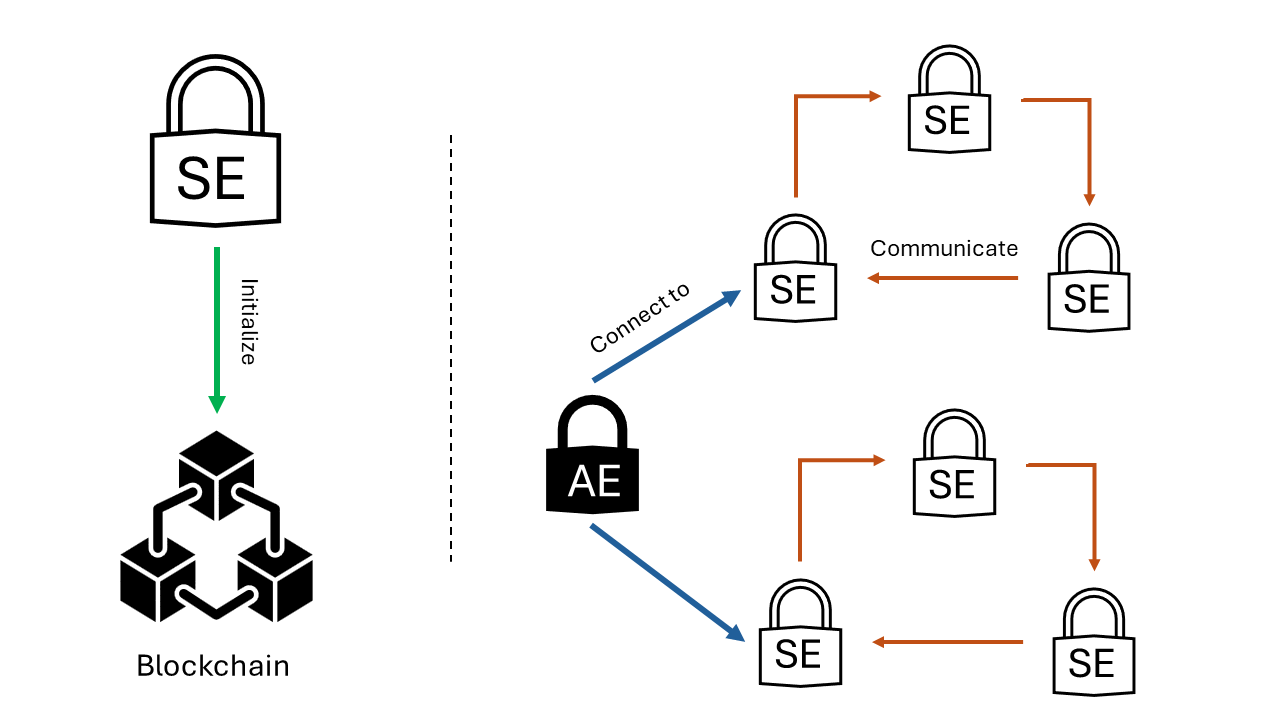
\includegraphics[width=\linewidth]{Figures/Figure1.png}
    \caption{The main components. The SE first has to initialize through the blockchain. Afterward, the groups will be established, where the AEs can link to}
    \label{fig:1}
\end{figure}


The authors also state a few premises which Narrator-Pro does. 
\begin{itemize}
    \item \textbf{Denial of Service Attacks} - It is not the goal to prevent systems from these kinds of attacks. Since TEEs themselves do not have prevention measures included.  
    \item \textbf{Hardware} - The implementation of Narrator-Pro should neither require any hardware changes nor will there be a need for specific hardware if the TEE is already implemented.  
    \item \textbf{No Trusted Central Party} - Narrator-Pro does not rely on Trusted central parties, like trusted servers. However, since an external blockchain is used to initialize the system, the authors can not state that their system does not rely on Trusted Third Parties.
\end{itemize} 

The main concepts that constitute the reliance on Narrator-Pro are §4.1 system initialization, §4.2 state update and read protocols for AEs, and §4.3 restart protocols regarding AEs and SEs.

\subsection{System Initialization}

Before the system can start processing requests, it is essential to initialize the SEs. Adversaries will not be able to launch SEs with the same binary in the same group to get stale states. This is accomplished by the usage of a blockchain \textit{B}. 

The blockchain \textit{B} serves to store tuples containing <\textit{key}, \textit{value}>. The \textit{value} is a random string linked to the \textit{key}, which will be returned by the blockchain in future read-calls. The, before mentioned, initialization process of SEs is carried out while the first write-call from a SE to \textit{B} is established. \textit{B} will verify that no other SE has registered on the blockchain with the provided \textit{key}. If this is the case the write-call will be executed and the client will receive an authenticator \textit{a}, with which he can verify the operation. This summarises the initialization responsibilities of \textit{B}.

The SE has to go through additional steps to finish its initialization. Therefore it is important to mention that SEs connect in groups to carry out requests delivered by AEs (Figure ~\ref{fig:1}). Every group has an SE leader who is responsible for storing certain information about the group. If an SE wants to initialize, it first lets the leader establish a secure connection to itself. This connection channel spreads through the whole group so the participants can talk to each other. After the channel is in place, the initializing SE creates a key pair (which will be used in future connection establishments with this SE) and sends it to the leader, where it will be collected and stored in a list that is accessible to every SE in the group. Afterward, the aforementioned blockchain interaction takes place where the SE performs a call to \textit{B} and either receives the \textit{value} containing \textit{Null} (stating that no other SE has already linked to it with this \textit{key}) and the initialization succeeds or the SE terminates its initialization process. Subsequently, the first write-call will be executed where the SE stores its <\textit{key}, \textit{value}> tuple, and only then it can proceed to process the AE request.

\subsection{State Update and Read}

To prevent eavesdropping from adversaries, messages between AEs and SEs are transmitted over encrypted channels, using secret session keys. A nonce (Number used once) is sent as well to prevent replays. An AE will use an aforementioned group of SEs to confirm its current state \(S_i\), before proceeding with input \(I_i\) to update to \(S_{i+1}\). The following paragraphs will explain this procedure further (\(SD_{i}\) refers to the state digest, which is a summary of the latest states):

\begin{enumerate}
    \item \textbf{Input} - After receiving \(I_i\) from a user, the AE saves a state snapshot <\(S_i\), \(I_i\), \(SD_{i-1}\)> on the disk, in case the process crashes midway, so the current input/state can be retrieved. The AEs next step is to call the function (\textbf{writeState(\(SD_i\))} -> ACK) and wait for the returning ACK from the SE, to proceed with the state update.
    \item \textbf{writeState()} - With calling the \textbf{writeState()} function, the SE saves a snapshot of its states, containing <\(S_j\), \(I_j\), \(SD_{j-1}\)> with \(I_j\) = \(SD_{i}\). Upon a successful save, the SE starts communicating with its group by sending a PREPARE message <Prepare, \(SD_{j}\), (\textit{j}, \textit{seq})> to all SEs.\\
    The tuple <(\textit{j}, \textit{seq})> will be used in §4.3 for a rebooting SE to indicate if an enclave is active or was displaced by its clone.
    \item \textbf{PREPARE message} - Receiving a PREPARE message triggers the SE to update the sending SEs state digest in their memory. Consequently, an ECHO message is sent, containing \(SD_{j}\), signaling a successful update to the sending SE. Upon receiving \textit{f} + 1 ECHO messages, the initial SE adds the new state \(S_{i+1}\) to \(SD_{j+1}\) and sends an ACK to the AE. It then will advance its state to \(S_{i+1}\) and send the corresponding output to the user.
\end{enumerate}

A similar approach is used when an AE wants to verify the freshness of its current state. It calls the \textbf{readState()} function of its connected SE. The target SE, however, can not just return its current state digest (containing the latest states, with the freshest on top)
since due to a forking attack there could be more than one instance of this SE, holding stale state digests. So the creators of Narrator-Pro developed a sequence this SE has to run through, to verify its freshness:
\begin{enumerate}
    \item After calling \textbf{readState()} the target SE sends a request to all SEs in the group to obtain their saved state digests.
    \item Each SE then sends back the saved state digest, corresponding to the target SE, since every SE holds a list of all SE state digests, in the group.
    \item The target SE has to receive at least \textit{f} + 1 replies, where the state digest is the same as its, to be able to return it to the AE. 
\end{enumerate}


\subsection{Restart Protocol}
The last vulnerability that was discovered by the creators of Narrator-Pro is when an SE reboots and reconnects to its group, an adversary can leverage the group to perform a certain sequence, to enable forking and rollback attacks. This fact is best explained with an example (Figure  ~\ref{fig:2}). Consider three SEs \(S_{1}\), \(S_{2}\) and \(S_{3}\). With cloning \(S_{1}\) -> \(S'_{1}\) and \(S_{2}\) -> \(S'_{2}\) the initial enclaves will be displaced in the group by their copies, leaving \(S_{1}\) and \(S_{2}\) to be inactive. \(S_{3}\) will now communicate with the clones. However, the enclaves \(S_{1}\) and \(S_{2}\) do not know that they are inactive, since the initial algorithm does not involve the necessity for the enclaves to know that they were displaced. Therefore a copy of \(S_{3}\) -> \(S'_{3}\) can link to \(S_{1}\) and \(S_{2}\). This leaves two groups, \textit{G1} and \textit{G2} of SEs. An adversary can now (1) increment the state with \textit{G1} and perform some actions leaving \textit{G2} with the old state, thereby rolling back the application. Or (2) feed two different inputs to \(S_{3}\) and \(S'_{3}\) and receive different outputs with 2 groups that have, respectfully the same binary, enabling a forking attack.\\
In order to prevent a system from performing this kind of sequence, the creators of Narrator-Pro included a requirement where an SE has to be confirmed by its group that at least \textit{f} SEs are not inactive, when reconnecting. This is accomplished by the tuple <(\textit{j}, \textit{seq})>, which is sent along with the \textbf{PREPARE messages}, where the index \textit{j} refers to the freshness of its state digest and \textit{seq} is used to distinguish different state digests with the same index.\\


\begin{figure}[h]
    \centering
    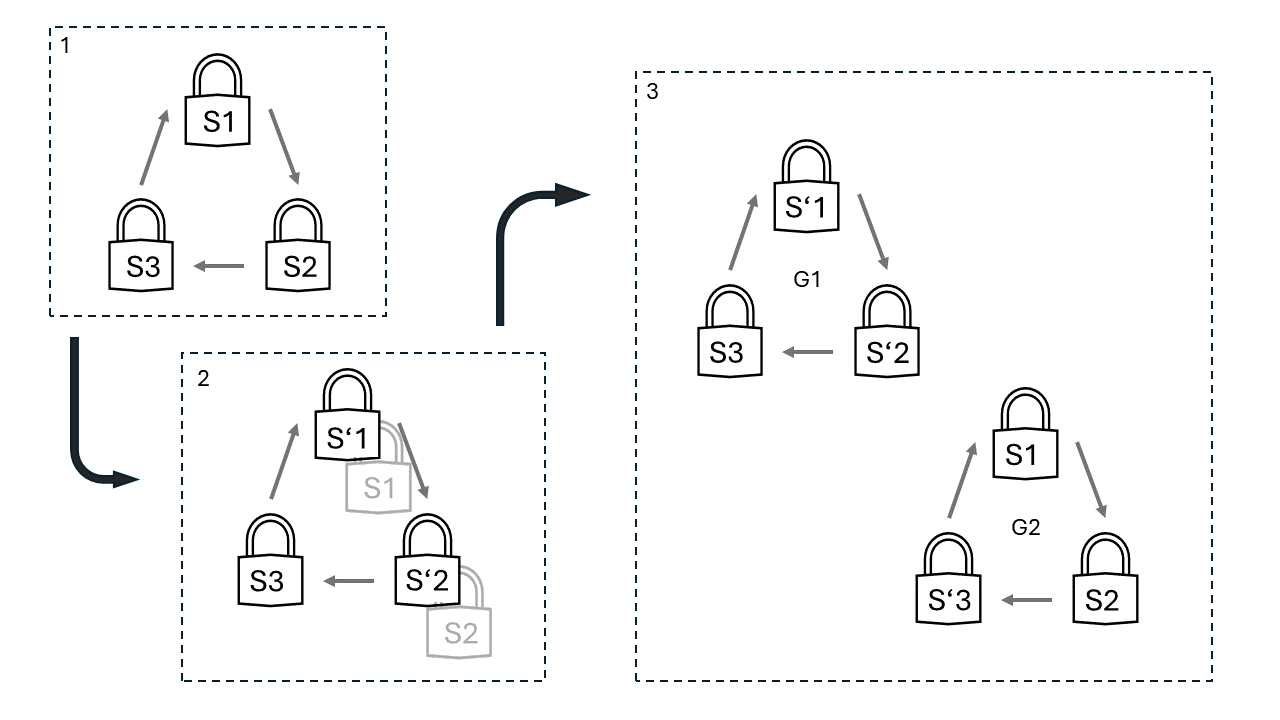
\includegraphics[width=\linewidth]{Figures/Figure2.png}
    \caption{The process of how to create forking groups}
    \label{fig:2}
\end{figure}

\section{Cache-based Channel - CloneBusters}
The uniqueness of CloneBusters~\cite{nfw} is the resignation of reliance on a Trusted Third Party (TTP) since they are hard to find in real-life applications. To achieve this goal they implemented a channel (respectfully a cache set) for every enclave in which only his binary can communicate in. This communication is then monitored by CloneBusters and fed to a classification algorithm to detect clones of an instance i.e. an enclave. \\
\\
\textbf{Clones} - If a second instance of an enclave is generated, it is set to be a clone if (i) they are loaded with the same binary and (ii) they run at the same time. (ii) is necessary since SGX itself can detect the clone if does not run simultaneously with the enclave. \\

The system relies on Monotonic Counters (MC) which will be incremented by an enclave to track its progress. The mode \textit{"inc-then-store"} is used which can be described as when data is stored, the index will be increased beforehand and then saved to deliver validation. This validation is carried out once, while storing the data so no index can be assigned to multiple data sets and second, if an enclave requests a data set it only accepts it if its counter is the same as the counter saved along with the data.\\
However, a vulnerability was discovered by the authors of CloneBusters while executing the \textit{"inc-then-store"} mode. Imagine one enclave E, its clone E', and a malicious OS that created that clone and is in control of the execution order of E and E'. Both enclaves will start with the same MC value (which is global) and loaded binary. In order to process Input \(I_1\), E increments MC once, however is then paused through the OS. The OS then feeds \(I_2\) to E' which also increments MC, leading MC to be +2. After that, the enclaves can proceed simultaneously since they will execute \textbf{Read(MC)} and receive the same value but arrive at different outputs which will be stored with the same index leading to a violation of the given rollback attack prevention from SGX. \\
Therefore CloneBusters developed a strategy to detect clones as they try to operate parallel to its enclave. The implementation of communication through already available cache sets enables CloneBusters to not rely on a TTP. This is accomplished by two phases which have to be executed, (1) the preparation phase and (2) the monitoring phase. The group of cache sets, i.e. the channel, is developed in (1) to enable phase (2) to monitor this channel where every instance with the same binary (the enclave and its clones) will put its data in, so a classification algorithm can check cache hits and misses to detect clones which will inevitably replace the data from the original enclave with its signed data.

\subsection{Preparation Phase (1)}
In order to assign cache sets to enclaves the creators of CloneBusters evaluated the physical addresses (16 Bits) of the system and concluded that these sets are best to be indexed by bits 6-15. This leaves a total of 16 cache sets which are used for a channel of an enclave. In the paper, they show that this is the perfect size for enclaves to detect the presence of clones.\\
After determining the right quantity, eviction sets have to be allocated to finalize the channels in which the enclaves will communicate in. The enclaves should have eviction sets where the memory is contiguous, however, the OS could assign non-contiguous memory. In order to avoid this violation, the creators developed an algorithm to create the eviction sets properly. The algorithm and its method of operation can be detailed in the paper.

\subsection{Monitoring Phase (2)}
With the establishment of the eviction sets the enclaves can start operating. CloneBusters has to run continuously while a critical phase is executed (e.g. while incrementing and reading the MC), to provide optimal security. Before entering the \textit{"inc-then-store"} section, the enclave has to pre-fetch, the data to be monitored, into the cache set to provide expressive reliance on CloneBusters. \\
The monitoring is done by measuring the time to access data on the cache. Since the enclave has to fetch its data into the cache, it expects to receive a cache hit if it accesses the data. However, if a clone is running simultaneously it will replace the enclave's data with its own, so the enclave will detect a cache miss. This recorded time is then forwarded to a classification algorithm. With a pre-defined threshold of what time it takes to access either cache hits or cache misses, the algorithm can distinguish them and determine if a clone is running. This information is then passed back to the enclave to take appropriate countermeasures like holding the execution.\\
The authors of CloneBusters note that the cache sets are used by other applications as well. Therefore they have provided evidence, that if the caches are polluted by different applications, CloneBusters will still operate in the expected way.

\section{Conclusion}
The reliance on TEE and enclaves provides confidentiality on data and secures executed programs within those enclaves. However, adversaries and malicious OS have found ways to mitigate this reliance by performing attacks on these sealed memory sections. Successful forking attacks on SGX-enabled systems have resulted in acknowledging the threat those systems deliver. Therefore the need for extensions on SGX increased and developers implemented systems that mitigate and prevent forking attacks from happening. 
The system, Narrator-Pro, decided to include a blockchain to initialize enclaves to prevent the launching of clones in the same group. Additional prevention is provided by protocols of state updates, that require SEs and AEs to confirm the freshness of their current state before evolving further. Finally, to ensure that no clone can connect with other groups the restart protocol was introduced.
This implementation delivers comprehensive rules for initialization, updates, and restarts, of enclaves. \\
CloneBusters on the other hand does not prevent clones from launching. It rather relies on defined cache sets in which every instance with the same binary (enclaves and their clones) has to fetch its data. This forces clones to replace data in the cache with their own, thereby enabling CloneBusters to measure cache hits and misses. This recorded data is then sent to a classification algorithm to detect if a clone is running. The cache-based communication is a comparatively simple implementation against forking attacks.\\
Those approaches contribute to the safety of TEEs, enable further development, and encourage the invention of other systems. 

\bibliography{Ref.bib}

\end{document}